Les dixièmes Rencontres Jeunes Chercheuses et Chercheurs en EIAH (RJC EIAH 2024) se sont tenues à Laval du 4 au 7 juin 2024. Ces rencontres sont une occasion particulièrement importante pour les jeunes chercheuses et chercheurs de la communauté EIAH (Environnements Informatiques pour l’Apprentissage Humain) de pouvoir se rencontrer et échanger avec des chercheuses et chercheurs autour de leurs travaux. 

En effet, les RJC EIAH, organisées tous les 2 ans sous l’égide de l’ATIEF (Association des Technologies de l'Information pour l'Éducation et la Formation) visent le développement de la communauté EIAH par la formation des doctorantes et doctorants issus des différentes disciplines inhérentes au domaine des EIAH et la diffusion de leurs travaux. 

\begin{figure}[!h]
	\centering
	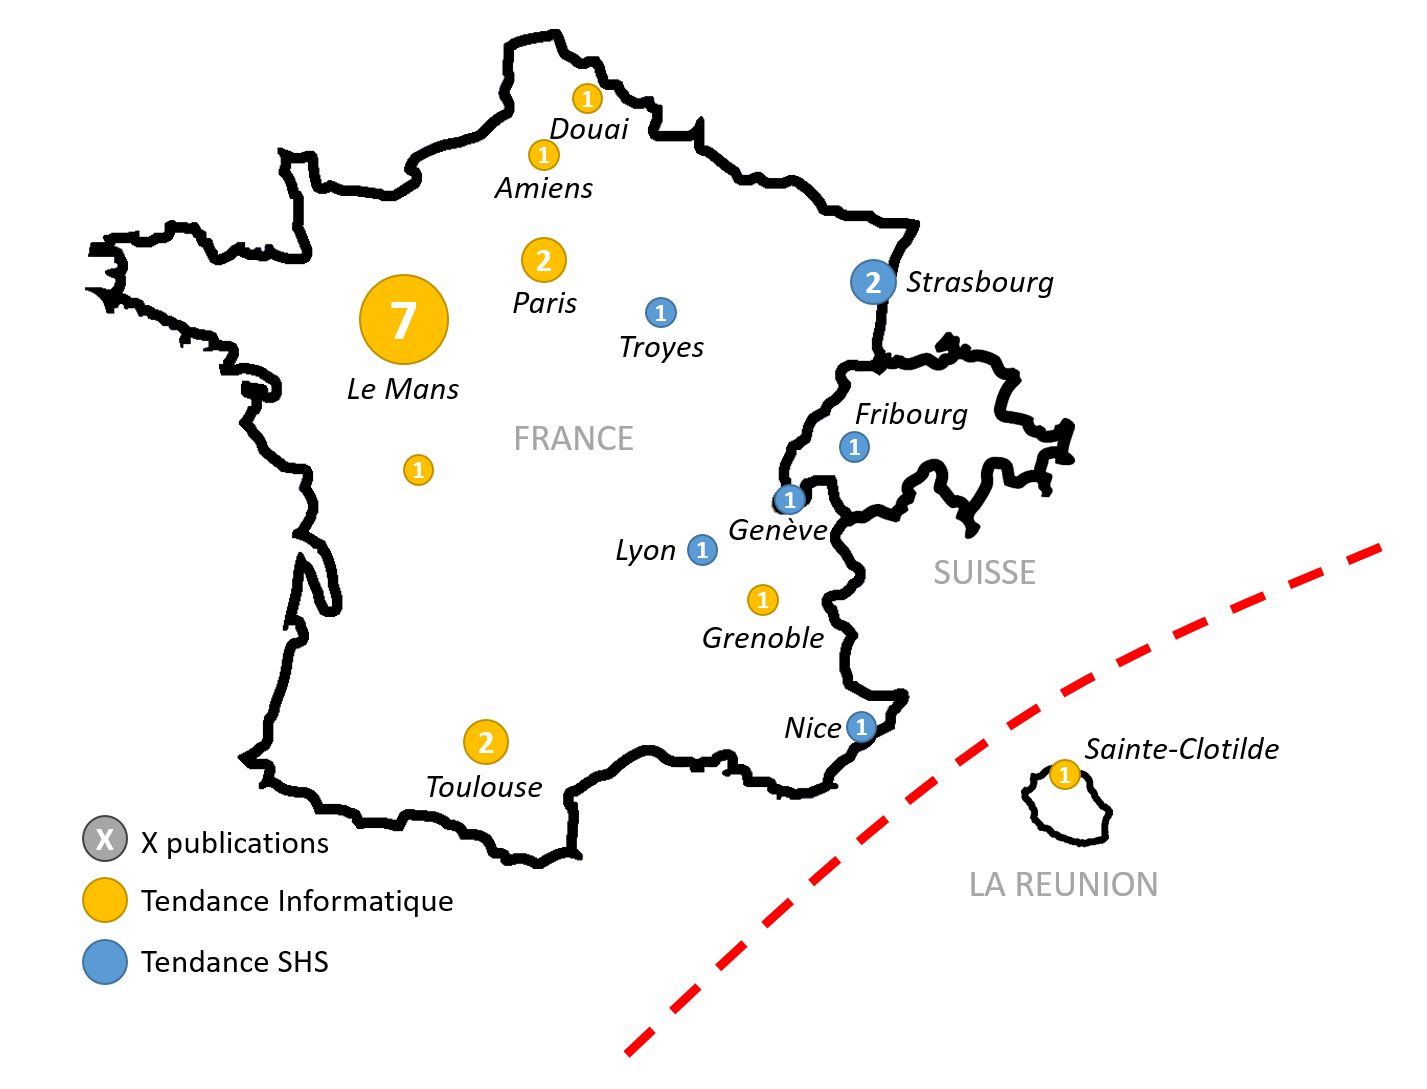
\includegraphics[width=0.7\textwidth]{Content/figures/carteComplete.png}
	\caption{Répartition géographique des publications des RJC EIAH 2024}
	\label{f:repGeoPubli}
\end{figure}

L’édition 2024 a retenu l’attention de 24 jeunes chercheuses et chercheurs qui ont soumis une contribution sous forme d’articles longs de 12 pages pour 17 d’entre eux, et d'articles courts de 4 pages pour 7 autres. 
Chacune des communications ont été évaluées par 2 membres du comité de programme issus pour l'un des sciences humaines et sociales (SHS) et pour l'autre de l'informatique. À l’issue de cette phase d'évaluation, 14 propositions ont été acceptées sous la forme d’articles longs, et 9 ont été acceptées sous la forme d’articles courts. Nous remercions d'ailleurs le comité de programme pour la qualité  des relectures et les commentaires conséquents et pédagogiques qui permettent l’amélioration des articles proposés et des présentations lors de la conférence.

Les articles longs acceptés ont été présentés lors de la conférence sous la forme d'une présentation orale et les articles courts à travers une présentation de poster.

Les contributions proviennent essentiellement d’universités françaises, mais comptent également des travaux issus de Suisse (2) (voir Figure \ref{f:repGeoPubli}). Les publications proviennent ainsi de 15 laboratoires de recherches différents.

\begin{figure}[!h]
	\centering
	\includegraphics[width=0.7\textwidth]{Content/figures/wordcloud.png}
	\caption{Nuage de mots des contributions à RJC-EIAH 2022}
	\label{f:wordCloud}
\end{figure}

Les contributions se répartissent entre les disciplines de l’informatique (14) et des sciences humaines et sociales (8). Pour cette édition, 2 grandes thématiques transversales aux disciplines ont été abordées par un grand nombre des travaux présentés~: près des trois quarts des contributions portent sur les formes d'apprentissage incluant majoritairement les jeux sérieux, la réalité virtuelle/augmentée/mixte et la simulation~; les travaux sur les usages sont également à l'honneur avec près de trois cinquièmes des articles, certains abordent la question sur l'axe des \textit{learning analytics} alors que d'autre sont orientés sur les modalités d'intégration et les méthodes d'évaluation. La figure \ref{f:wordCloud} qui expose les termes les plus présents dans les contributions fait état de ces tendances.

Ces contributions ont donc fait l’objet de quatre sessions distinctes : 
\begin{enumerate}
	\item Analyse d'usage(s) et de pratiques ;
	\item Méthodes d'évaluation des dispositifs d'apprentissage / de formation dans les EIAH ;
	\item Méthodes de conception des EIAH et Systèmes adaptatifs et personnalisation de l'apprentissage ;
	\item Modalités d'organisation communautaires (collaboration, coopération...).
\end{enumerate}

Ces rencontres jeunes chercheur.e.s ont également accueilli une conférence de la Professeur ... de l'Université ..., qui porte sur ... ; aussi nous la remercions chaleureusement.

Nous remercions aussi l’ATIEF, les différents membres des comités de programme, d'organisation et de coordination des ateliers ainsi que les différents partenaires pour leur soutien à cette manifestation et plus particulièrement l’Université du Mans qui a accueilli les rencontres sur son site de Laval.

Pour finir, nous remercions chaleureusement tous les chercheurs en EIAH, et en particulier les jeunes chercheuses et chercheurs sans qui ces rencontres n’auraient pas lieu.

\vspace*{2em}
\begin{flushright}
	Sonia Mandin et Mathieu Muratet, co-présidents du comité de programme
\end{flushright}